\PassOptionsToPackage{unicode=true}{hyperref} % options for packages loaded elsewhere
\PassOptionsToPackage{hyphens}{url}
%
\documentclass[12pt,]{article}
\usepackage{lmodern}
\usepackage{amssymb,amsmath}
\usepackage{ifxetex,ifluatex}
\usepackage{fixltx2e} % provides \textsubscript
\ifnum 0\ifxetex 1\fi\ifluatex 1\fi=0 % if pdftex
  \usepackage[T1]{fontenc}
  \usepackage[utf8]{inputenc}
  \usepackage{textcomp} % provides euro and other symbols
\else % if luatex or xelatex
  \usepackage{unicode-math}
  \defaultfontfeatures{Ligatures=TeX,Scale=MatchLowercase}
    \setmainfont[]{Times New Roman}
\fi
% use upquote if available, for straight quotes in verbatim environments
\IfFileExists{upquote.sty}{\usepackage{upquote}}{}
% use microtype if available
\IfFileExists{microtype.sty}{%
\usepackage[]{microtype}
\UseMicrotypeSet[protrusion]{basicmath} % disable protrusion for tt fonts
}{}
\IfFileExists{parskip.sty}{%
\usepackage{parskip}
}{% else
\setlength{\parindent}{0pt}
\setlength{\parskip}{6pt plus 2pt minus 1pt}
}
\usepackage{hyperref}
\hypersetup{
            pdftitle={Central Appalachian Mine Closures},
            pdfauthor={Hannah Smith},
            pdfborder={0 0 0},
            breaklinks=true}
\urlstyle{same}  % don't use monospace font for urls
\usepackage[margin=2.54cm]{geometry}
\usepackage{color}
\usepackage{fancyvrb}
\newcommand{\VerbBar}{|}
\newcommand{\VERB}{\Verb[commandchars=\\\{\}]}
\DefineVerbatimEnvironment{Highlighting}{Verbatim}{commandchars=\\\{\}}
% Add ',fontsize=\small' for more characters per line
\usepackage{framed}
\definecolor{shadecolor}{RGB}{248,248,248}
\newenvironment{Shaded}{\begin{snugshade}}{\end{snugshade}}
\newcommand{\AlertTok}[1]{\textcolor[rgb]{0.94,0.16,0.16}{#1}}
\newcommand{\AnnotationTok}[1]{\textcolor[rgb]{0.56,0.35,0.01}{\textbf{\textit{#1}}}}
\newcommand{\AttributeTok}[1]{\textcolor[rgb]{0.77,0.63,0.00}{#1}}
\newcommand{\BaseNTok}[1]{\textcolor[rgb]{0.00,0.00,0.81}{#1}}
\newcommand{\BuiltInTok}[1]{#1}
\newcommand{\CharTok}[1]{\textcolor[rgb]{0.31,0.60,0.02}{#1}}
\newcommand{\CommentTok}[1]{\textcolor[rgb]{0.56,0.35,0.01}{\textit{#1}}}
\newcommand{\CommentVarTok}[1]{\textcolor[rgb]{0.56,0.35,0.01}{\textbf{\textit{#1}}}}
\newcommand{\ConstantTok}[1]{\textcolor[rgb]{0.00,0.00,0.00}{#1}}
\newcommand{\ControlFlowTok}[1]{\textcolor[rgb]{0.13,0.29,0.53}{\textbf{#1}}}
\newcommand{\DataTypeTok}[1]{\textcolor[rgb]{0.13,0.29,0.53}{#1}}
\newcommand{\DecValTok}[1]{\textcolor[rgb]{0.00,0.00,0.81}{#1}}
\newcommand{\DocumentationTok}[1]{\textcolor[rgb]{0.56,0.35,0.01}{\textbf{\textit{#1}}}}
\newcommand{\ErrorTok}[1]{\textcolor[rgb]{0.64,0.00,0.00}{\textbf{#1}}}
\newcommand{\ExtensionTok}[1]{#1}
\newcommand{\FloatTok}[1]{\textcolor[rgb]{0.00,0.00,0.81}{#1}}
\newcommand{\FunctionTok}[1]{\textcolor[rgb]{0.00,0.00,0.00}{#1}}
\newcommand{\ImportTok}[1]{#1}
\newcommand{\InformationTok}[1]{\textcolor[rgb]{0.56,0.35,0.01}{\textbf{\textit{#1}}}}
\newcommand{\KeywordTok}[1]{\textcolor[rgb]{0.13,0.29,0.53}{\textbf{#1}}}
\newcommand{\NormalTok}[1]{#1}
\newcommand{\OperatorTok}[1]{\textcolor[rgb]{0.81,0.36,0.00}{\textbf{#1}}}
\newcommand{\OtherTok}[1]{\textcolor[rgb]{0.56,0.35,0.01}{#1}}
\newcommand{\PreprocessorTok}[1]{\textcolor[rgb]{0.56,0.35,0.01}{\textit{#1}}}
\newcommand{\RegionMarkerTok}[1]{#1}
\newcommand{\SpecialCharTok}[1]{\textcolor[rgb]{0.00,0.00,0.00}{#1}}
\newcommand{\SpecialStringTok}[1]{\textcolor[rgb]{0.31,0.60,0.02}{#1}}
\newcommand{\StringTok}[1]{\textcolor[rgb]{0.31,0.60,0.02}{#1}}
\newcommand{\VariableTok}[1]{\textcolor[rgb]{0.00,0.00,0.00}{#1}}
\newcommand{\VerbatimStringTok}[1]{\textcolor[rgb]{0.31,0.60,0.02}{#1}}
\newcommand{\WarningTok}[1]{\textcolor[rgb]{0.56,0.35,0.01}{\textbf{\textit{#1}}}}
\usepackage{graphicx,grffile}
\makeatletter
\def\maxwidth{\ifdim\Gin@nat@width>\linewidth\linewidth\else\Gin@nat@width\fi}
\def\maxheight{\ifdim\Gin@nat@height>\textheight\textheight\else\Gin@nat@height\fi}
\makeatother
% Scale images if necessary, so that they will not overflow the page
% margins by default, and it is still possible to overwrite the defaults
% using explicit options in \includegraphics[width, height, ...]{}
\setkeys{Gin}{width=\maxwidth,height=\maxheight,keepaspectratio}
\setlength{\emergencystretch}{3em}  % prevent overfull lines
\providecommand{\tightlist}{%
  \setlength{\itemsep}{0pt}\setlength{\parskip}{0pt}}
\setcounter{secnumdepth}{5}
% Redefines (sub)paragraphs to behave more like sections
\ifx\paragraph\undefined\else
\let\oldparagraph\paragraph
\renewcommand{\paragraph}[1]{\oldparagraph{#1}\mbox{}}
\fi
\ifx\subparagraph\undefined\else
\let\oldsubparagraph\subparagraph
\renewcommand{\subparagraph}[1]{\oldsubparagraph{#1}\mbox{}}
\fi

% set default figure placement to htbp
\makeatletter
\def\fps@figure{htbp}
\makeatother

\usepackage{etoolbox}
\makeatletter
\providecommand{\subtitle}[1]{% add subtitle to \maketitle
  \apptocmd{\@title}{\par {\large #1 \par}}{}{}
}
\makeatother

\title{Central Appalachian Mine Closures}
\providecommand{\subtitle}[1]{}
\subtitle{\url{https://github.com/hgs13/EDA_Final_Project_2020}}
\author{Hannah Smith}
\date{}

\begin{document}
\maketitle

\newpage
\tableofcontents 
\newpage
\listoftables 
\newpage
\listoffigures 
\newpage

\hypertarget{rationale-and-research-questions}{%
\section{Rationale and Research
Questions}\label{rationale-and-research-questions}}

This project seeks to analyze preliminary data that may affect the
migration patterns of residents of coal counties in central Appalachia
from the years 2000 to 2011. There is little to no research exploring
migration patterns in Appalachia during this time period, especially as
it relates to migration. Furthermore, the energy sector is transitioning
to greener energy, which further impacts coal production, especially in
Appalachia.

Two ``coal counties'' serve as a case study for migration in central
Appalachia: Harlan County, Kentucky and Dickenson County, Virginia.
Harlan County serves as a ``Boom-Bust'' county, meaning the county
experienced a coal production boom in 2000 and a coal production bust in
2010. Dickenson, on the other hand, is a ``Bust-Bust'' county, where the
county experienced a coal production bust in 2000 and did not recover by
2010.

An important portion of understanding migration in Appalachia is
investigating the mine operations within the coal counties. As such,
this project creates and analyzes a visualization of mine production and
employment in Harlan and Dickenson counties between the years 2000 and
2011. The data analysis of the coal production and the number of
employees in coal mines in each county could be indicative of migration
patterns within the central Appalachian region.

The main questions for this research study are as follows:

\begin{enumerate}
\def\labelenumi{\arabic{enumi}.}
\tightlist
\item
  What is the relationship between coal production and number of
  employees in coal mines in Harlan and Dickenson Counties?
\end{enumerate}

\begin{enumerate}
\def\labelenumi{\alph{enumi}.}
\item
  How does coal production differ between all mines in Harlan County
  compared to Dickenson County?
\item
  How does the number of employees in the mines of Harlan County compare
  to Dickenson County?
\item
  Is the total number of employees for all mines in a boom-bust and a
  bust-bust county in the years 2000 to 2011 a significant predictor of
  annual coal production for all mines?
\end{enumerate}

\newpage

\hypertarget{dataset-information}{%
\section{Dataset Information}\label{dataset-information}}

\hypertarget{data-origin-location}{%
\subsection{Data Origin Location}\label{data-origin-location}}

The data in this repository is coal mine data compiled by the Coal and
America Bass Connections team at Duke University from the Energy
Information Administration (EIA) online database throughout the fall of
2019. The data in this repository is coal mine data compiled by the Coal
and America Bass Connections team at Duke University from the Energy
Information Administration (EIA) online database throughout the fall of
2019.

"This report is mandatory under the Federal Energy Administration Act of
1974 (Public Law 93-275). Failure to comply may result in criminal
fines, civil penalties, and other sanctions as provided by law. Title 18
USC 1001 makes it a criminal offense for any person knowingly and
willingly to make to any Agency or Department of the United States any
false, fictitious, or fraudulent statements as to any matter within its
jurisdiction.

All coal mining companies that owned a mining operation which produced
25,000 or more short tons of coal during the reporting year must submit
form EIA-7A, except for anthracite mines. All anthracite mines that
produced 10,000 or more short tons during the reporting year must submit
form EIA-7A. Standalone facilities (e.g., preparation
plant/tipple/loading dock/train loadout) that worked 5,000 or more hours
must submit the EIA-7A. Submit a separate form EIA-7A for each mining
operation and standalone facility that meets the reporting criteria.

The U.S. Energy Information Administration's (EIA) Form EIA-7A, Annual
Survey of Coal Production and Preparation, collects coal production data
from U.S. coal mining companies. This includes information on the type
and status of coal operations, characteristics of coalbeds mined,
recoverable reserves, productive capacity and the disposition of coal
mined which provides Congress with basic statistics concerning coal
supply. These data appear in the Annual Coal Report, the Quarterly Coal
Report, the Monthly Energy Review, and the Annual Energy Review. In
addition, the EIA uses the data for coal supply analyses and in
short-term modeling efforts, which produce forecasts of coal supply and
prices requested by Congress. The forecast data also appear in the
Short-Term Energy Outlook and the Annual Energy Outlook." (EIA, Form
EIA-7A)

Therefore, the data used in this project should be timely and accurate.
Furthermore, coal production during the decade this project explores was
extremely variable. As such, there should be no exclusion of outliers in
this report.

\hypertarget{data-wrangling-methods}{%
\subsection{Data Wrangling Methods}\label{data-wrangling-methods}}

For this project, the data was imported as two separate .csv files for
each county of interest (Harlan, Kentucky and Dickenson, Virginia). From
there, each column was coerced into the appropriate vector format. The
two data frames were then joined into one data frame to create ease of
access. Then, irrelevant columns were removed so that only the year,
mine name, mine state, mine county, mine status, operation type,
operating company, average employees, and labor hours were included.
After this, only active mines were selected for, as inactive mines would
skew the data. After grouping the remaining data by year and county, the
total production, total employed, mean production, and mean empoyment
were found for each county by year.

\hypertarget{data-exploration}{%
\subsection{Data Exploration}\label{data-exploration}}

Data exploration of the Harlan and Dickenson County raw data files

\begin{Shaded}
\begin{Highlighting}[]
\KeywordTok{dim}\NormalTok{(harlan.raw)}
\end{Highlighting}
\end{Shaded}

\begin{verbatim}
## [1] 509  15
\end{verbatim}

\begin{Shaded}
\begin{Highlighting}[]
\KeywordTok{dim}\NormalTok{(dickenson.raw)}
\end{Highlighting}
\end{Shaded}

\begin{verbatim}
## [1] 194  15
\end{verbatim}

\begin{Shaded}
\begin{Highlighting}[]
\KeywordTok{str}\NormalTok{(harlan.raw)}
\end{Highlighting}
\end{Shaded}

\begin{verbatim}
## 'data.frame':    509 obs. of  15 variables:
##  $ year                     : int  2011 2011 2011 2011 2011 2011 2011 2011 2011 2011 ...
##  $ mine.name                : Factor w/ 126 levels "# 1","# 2","# 3",..: 34 104 122 46 41 91 47 14 86 39 ...
##  $ mine.state               : Factor w/ 1 level "Kentucky (East)": 1 1 1 1 1 1 1 1 1 1 ...
##  $ countystr                : Factor w/ 1 level "Harlan": 1 1 1 1 1 1 1 1 1 1 ...
##  $ mine.basin               : Factor w/ 1 level "Appalachia Central": 1 1 1 1 1 1 1 1 1 1 ...
##  $ mine.status              : Factor w/ 6 levels "Active","Active, men not working, not producing",..: 1 1 1 1 1 1 1 1 1 1 ...
##  $ mine.type                : Factor w/ 1 level "Underground": 1 1 1 1 1 1 1 1 1 1 ...
##  $ company.type             : Factor w/ 3 levels "Contractor","Indepedent Producer Operator",..: 2 2 2 2 2 2 2 2 2 2 ...
##  $ operation.type           : Factor w/ 2 levels "Mine only","Preparation Plant": 1 2 2 2 2 2 1 2 1 2 ...
##  $ operating.company        : Factor w/ 102 levels "A & M Coal Co Inc",..: 54 64 37 37 31 76 54 69 46 54 ...
##  $ operating.company.address: Factor w/ 92 levels "1160 Jackson Dr, Paris, TN 38242",..: 33 21 59 59 58 50 33 48 57 33 ...
##  $ production.stons         : Factor w/ 400 levels "0","1,013,140",..: 248 1 1 1 1 1 313 1 81 1 ...
##  $ average.employees        : int  110 25 22 20 2 9 127 2 35 4 ...
##  $ labor.hours              : Factor w/ 468 levels "","1,211","1,692",..: 174 243 365 380 302 92 193 298 446 8 ...
##  $ ARC                      : int  1 1 1 1 1 1 1 1 1 1 ...
\end{verbatim}

\begin{Shaded}
\begin{Highlighting}[]
\KeywordTok{str}\NormalTok{(dickenson.raw)}
\end{Highlighting}
\end{Shaded}

\begin{verbatim}
## 'data.frame':    194 obs. of  15 variables:
##  $ year                     : int  2011 2011 2011 2011 2011 2011 2011 2011 2011 2011 ...
##  $ mine.name                : Factor w/ 56 levels "#1","#2","#44",..: 37 16 36 32 11 10 17 6 50 55 ...
##  $ mine.state               : Factor w/ 1 level "Virginia": 1 1 1 1 1 1 1 1 1 1 ...
##  $ countystr                : Factor w/ 1 level "Dickenson": 1 1 1 1 1 1 1 1 1 1 ...
##  $ mine.basin               : Factor w/ 1 level "Appalachia Central": 1 1 1 1 1 1 1 1 1 1 ...
##  $ mine.status              : Factor w/ 5 levels "Active","Active, men working, not producing",..: 1 1 1 1 1 1 1 1 1 2 ...
##  $ mine.type                : Factor w/ 1 level "Underground": 1 1 1 1 1 1 1 1 1 1 ...
##  $ company.type             : Factor w/ 3 levels "Contractor","Indepedent Producer Operator",..: 2 2 2 2 2 2 3 3 3 2 ...
##  $ operation.type           : Factor w/ 2 levels "Mine only","Preparation Plant": 1 1 1 1 1 1 2 1 1 2 ...
##  $ operating.company        : Factor w/ 57 levels "Apple Jacks Coal Company Inc",..: 8 26 13 30 46 46 23 22 22 19 ...
##  $ operating.company.address: Factor w/ 61 levels "1229 Homecreek Rd., Big Rock, VA 24202",..: 24 21 24 26 5 5 4 4 8 28 ...
##  $ production.stons         : Factor w/ 163 levels "0","1,719","103,817",..: 87 118 74 96 52 121 1 48 27 1 ...
##  $ average.employees        : int  16 17 13 14 94 48 37 101 36 7 ...
##  $ labor.hours              : Factor w/ 168 levels "","1,689","101,738",..: 97 127 84 82 58 168 158 56 162 32 ...
##  $ ARC                      : int  1 1 1 1 1 1 1 1 1 1 ...
\end{verbatim}

\begin{Shaded}
\begin{Highlighting}[]
\KeywordTok{colnames}\NormalTok{(harlan.raw)}
\end{Highlighting}
\end{Shaded}

\begin{verbatim}
##  [1] "year"                      "mine.name"                
##  [3] "mine.state"                "countystr"                
##  [5] "mine.basin"                "mine.status"              
##  [7] "mine.type"                 "company.type"             
##  [9] "operation.type"            "operating.company"        
## [11] "operating.company.address" "production.stons"         
## [13] "average.employees"         "labor.hours"              
## [15] "ARC"
\end{verbatim}

\begin{Shaded}
\begin{Highlighting}[]
\KeywordTok{colnames}\NormalTok{(dickenson.raw)}
\end{Highlighting}
\end{Shaded}

\begin{verbatim}
##  [1] "year"                      "mine.name"                
##  [3] "mine.state"                "countystr"                
##  [5] "mine.basin"                "mine.status"              
##  [7] "mine.type"                 "company.type"             
##  [9] "operation.type"            "operating.company"        
## [11] "operating.company.address" "production.stons"         
## [13] "average.employees"         "labor.hours"              
## [15] "ARC"
\end{verbatim}

\begin{Shaded}
\begin{Highlighting}[]
\KeywordTok{summary}\NormalTok{(harlan.raw)}
\end{Highlighting}
\end{Shaded}

\begin{verbatim}
##       year                mine.name             mine.state   countystr  
##  Min.   :2000   Mine #1        : 24   Kentucky (East):509   Harlan:509  
##  1st Qu.:2003   Prep Plant     : 21                                     
##  Median :2006   Mine No 1      : 19                                     
##  Mean   :2006   Mine No. 1     : 11                                     
##  3rd Qu.:2008   No 1 Plant     : 11                                     
##  Max.   :2011   Darby Fork No 1: 10                                     
##                 (Other)        :413                                     
##               mine.basin                                  mine.status 
##  Appalachia Central:509   Active                                :420  
##                           Active, men not working, not producing:  1  
##                           Active, men working, not producing    : 34  
##                           Mine closed by MSHA                   : 21  
##                           Permanently abandoned                 : 27  
##                           Temporarily closed                    :  6  
##                                                                       
##        mine.type                         company.type           operation.type
##  Underground:509   Contractor                  : 92   Mine only        :399   
##                    Indepedent Producer Operator:324   Preparation Plant:110   
##                    Operating Subsidiary        : 93                           
##                                                                               
##                                                                               
##                                                                               
##                                                                               
##                       operating.company
##  Harlan Cumberland Coal Company: 46    
##  Lone Mountain Processing Inc  : 31    
##  Manalapan Mining Co., Inc.    : 29    
##  Manalapan Mining Company Inc  : 28    
##  Liggett Mining Llc            : 23    
##  Rex Coal Company, Inc.        : 14    
##  (Other)                       :338    
##                           operating.company.address  production.stons
##  P.O. Box 269, Grays Knob, KY 40829    : 42         0        :110    
##  P.O. Box 527, Benham, KY 40807        : 35         1,013,140:  1    
##  8174 E Hwy 72, Pathfork, KY 40863     : 31         1,046,339:  1    
##  P.O. Box 838, Middlesboro, KY 40965   : 28         1,047,698:  1    
##  P.O. Box 1226, Norton, VA 24273       : 25         1,122,057:  1    
##  General Delivery, Grays Knob, KY 40829: 22         1,186,166:  1    
##  (Other)                               :326         (Other)  :394    
##  average.employees  labor.hours       ARC   
##  Min.   :  1.00           : 40   Min.   :1  
##  1st Qu.: 15.00    23,520 :  3   1st Qu.:1  
##  Median : 25.00    1,211  :  1   Median :1  
##  Mean   : 34.83    1,692  :  1   Mean   :1  
##  3rd Qu.: 40.00    1,702  :  1   3rd Qu.:1  
##  Max.   :166.00    1,705  :  1   Max.   :1  
##  NA's   :40        (Other):462
\end{verbatim}

\begin{Shaded}
\begin{Highlighting}[]
\KeywordTok{summary}\NormalTok{(dickenson.raw)}
\end{Highlighting}
\end{Shaded}

\begin{verbatim}
##       year                      mine.name      mine.state      countystr  
##  Min.   :2000   Cherokee Mine        : 12   Virginia:194   Dickenson:194  
##  1st Qu.:2001   Mc Clure River  Plant: 10                                 
##  Median :2004   Nme                  :  8                                 
##  Mean   :2005   No 8                 :  7                                 
##  3rd Qu.:2007   No. 3 Mine           :  7                                 
##  Max.   :2011   No. 4                :  7                                 
##                 (Other)              :143                                 
##               mine.basin                              mine.status 
##  Appalachia Central:194   Active                            :151  
##                           Active, men working, not producing: 14  
##                           Mine closed by MSHA               :  4  
##                           Permanently abandoned             : 21  
##                           Temporarily closed                :  4  
##                                                                   
##                                                                   
##        mine.type                         company.type           operation.type
##  Underground:194   Contractor                  :50    Mine only        :162   
##                    Indepedent Producer Operator:66    Preparation Plant: 32   
##                    Operating Subsidiary        :78                            
##                                                                               
##                                                                               
##                                                                               
##                                                                               
##                       operating.company
##  DickensonRussell Coal Company : 19    
##  Clinchfield Coal Company      : 12    
##  DickensonRussell Coal Co Llc  :  9    
##  L & J Equipment Company       :  9    
##  Apple Jacks Coal Company, Inc.:  7    
##  DickensonRussell Coal Co., Ll :  7    
##  (Other)                       :131    
##                          operating.company.address production.stons
##  P.O. Box 1426, Grundy, VA 24614      : 15         0      : 32     
##  5703 Crutchfield Dr, Norton, VA 24273: 11         1,719  :  1     
##  P.O. Box 1025, Grundy, VA 24614      :  9         103,817:  1     
##  P.O. Box 148, Vansant, VA 24656      :  8         104,108:  1     
##  P.O. Box 458, Big Rock, VA 24603     :  8         104,515:  1     
##  Rt 2, Box 73, Cleveland, VA 24225    :  8         109,076:  1     
##  (Other)                              :135         (Other):157     
##  average.employees  labor.hours       ARC   
##  Min.   :  1.00           : 26   Min.   :1  
##  1st Qu.: 12.00    79,091 :  2   1st Qu.:1  
##  Median : 16.00    1,689  :  1   Median :1  
##  Mean   : 30.11    101,738:  1   Mean   :1  
##  3rd Qu.: 40.00    104,181:  1   3rd Qu.:1  
##  Max.   :117.00    107,901:  1   Max.   :1  
##  NA's   :26        (Other):162
\end{verbatim}

\newpage

\hypertarget{exploratory-analysis}{%
\section{Exploratory Analysis}\label{exploratory-analysis}}

\hypertarget{visual-data-exploration-of-harlan-and-dickenson-data}{%
\subsection{Visual Data Exploration of Harlan and Dickenson
Data}\label{visual-data-exploration-of-harlan-and-dickenson-data}}

\begin{figure}
\centering
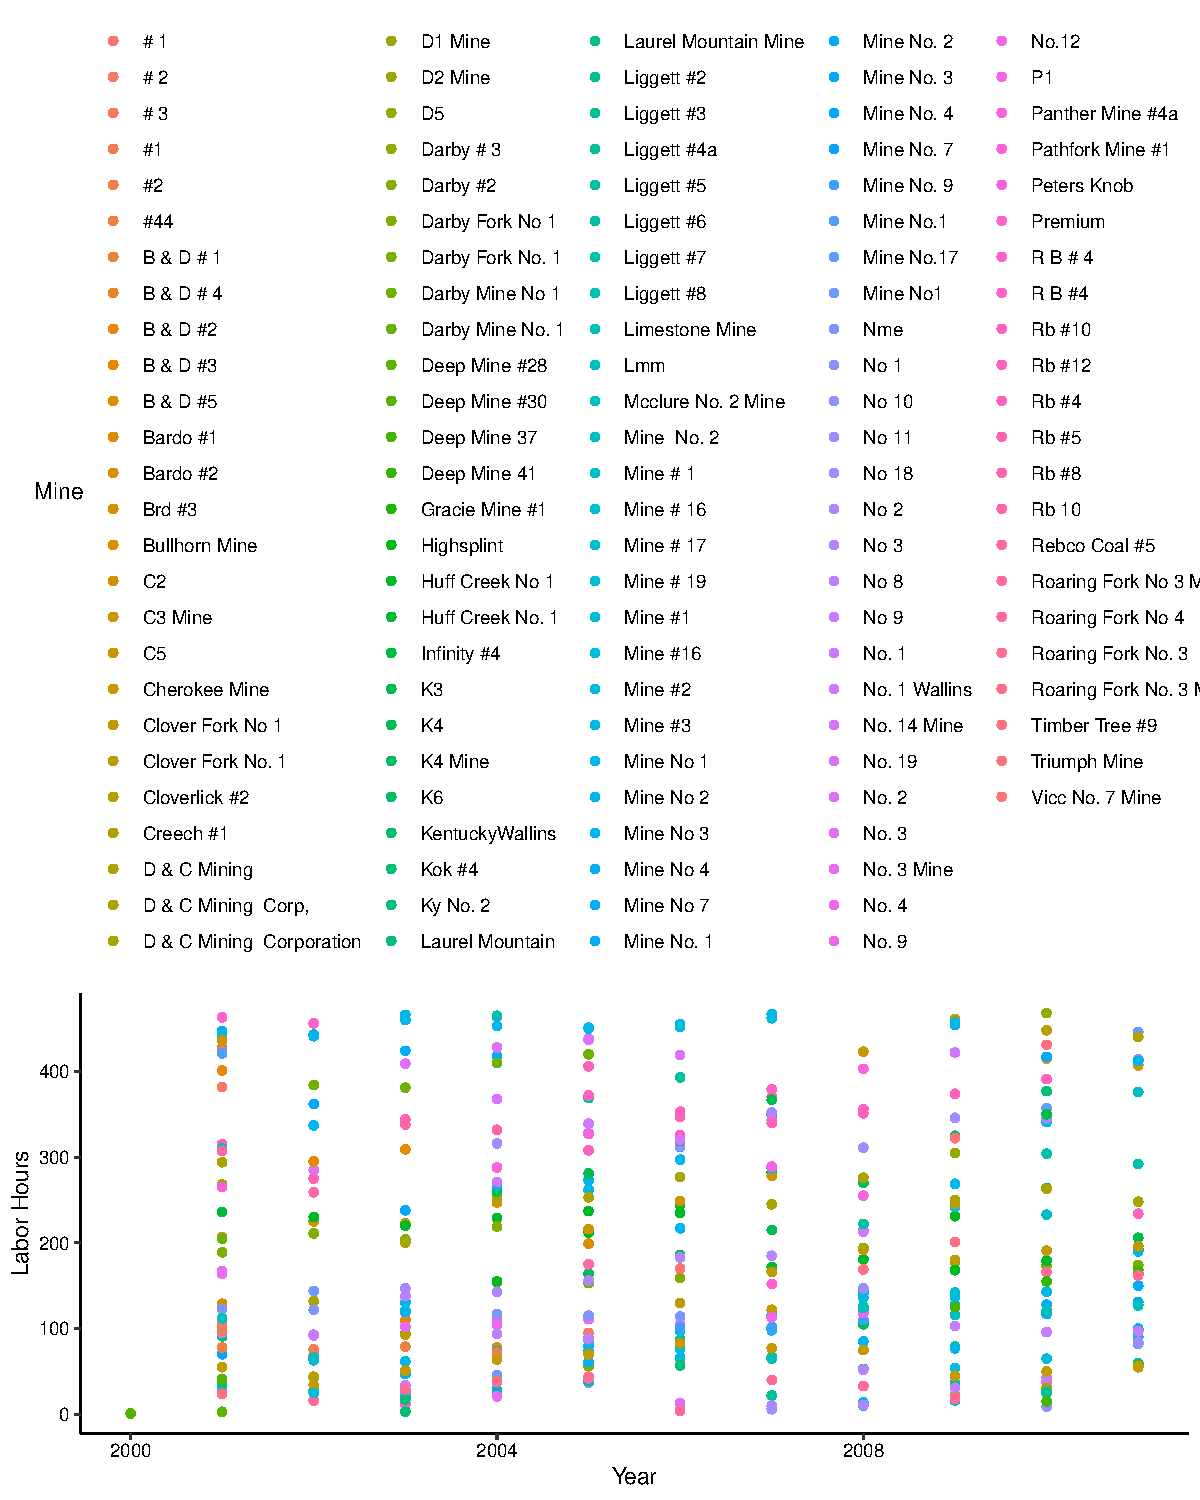
\includegraphics{Smith_ENV872_Project_files/figure-latex/unnamed-chunk-6-1.pdf}
\caption{\label{fig:figs} Total Annual Labor Hours for Mining in Harlan
and Dickenson Counties by Mine}
\end{figure}

\begin{figure}
\centering
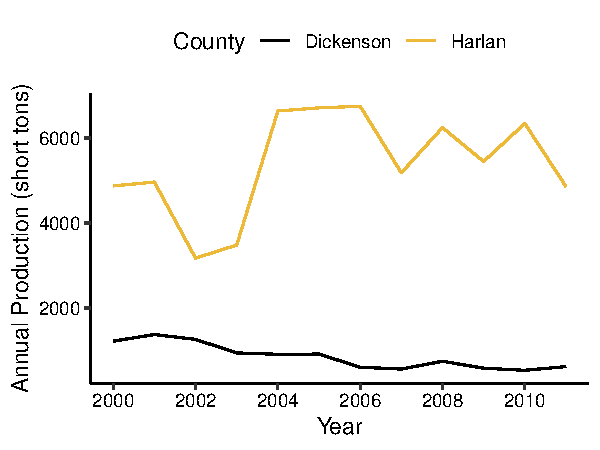
\includegraphics{Smith_ENV872_Project_files/figure-latex/unnamed-chunk-7-1.pdf}
\caption{\label{fig:figs} Total Annual Labor Hours for Mining in Harlan
and Dickenson Counties by County}
\end{figure}

\begin{figure}
\centering
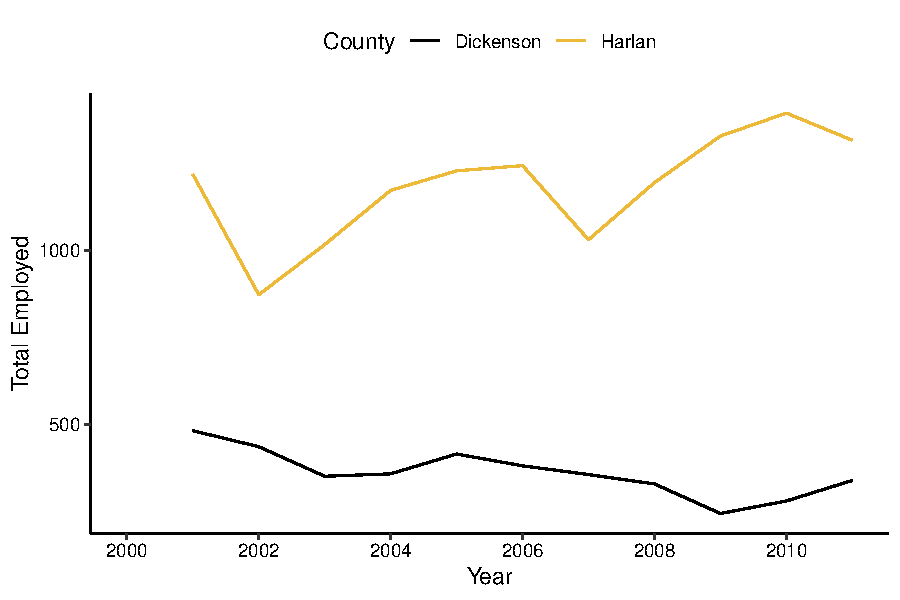
\includegraphics{Smith_ENV872_Project_files/figure-latex/unnamed-chunk-8-1.pdf}
\caption{\label{fig:figs} Total Annual Coal Employment in Harlan and
Dickenson Counties by Mine}
\end{figure}

\begin{figure}
\centering
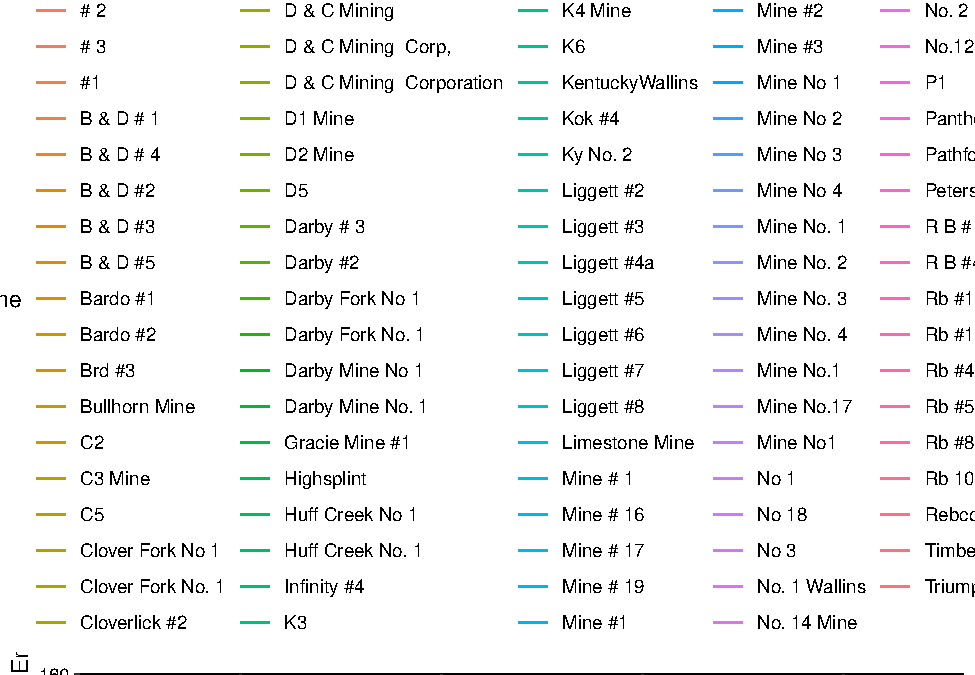
\includegraphics{Smith_ENV872_Project_files/figure-latex/unnamed-chunk-9-1.pdf}
\caption{\label{fig:figs} Total Annual Coal Employment in Harlan and
Dickenson Counties by County}
\end{figure}

\begin{figure}
\centering
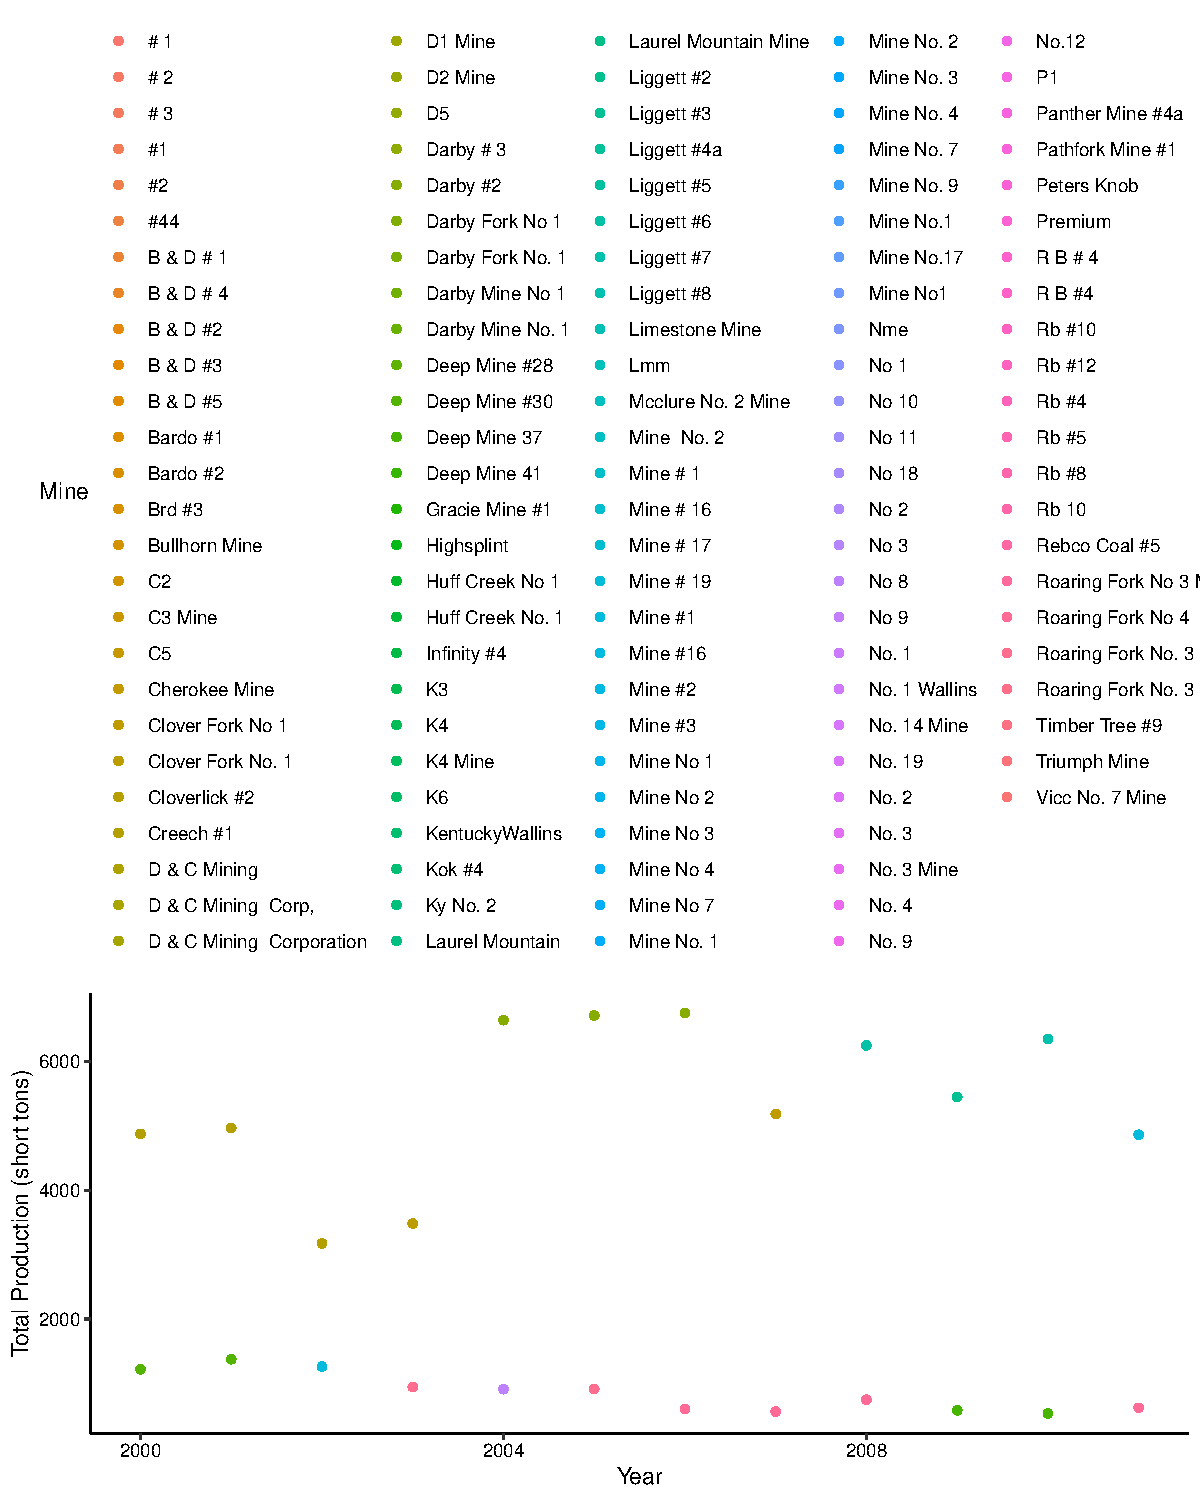
\includegraphics{Smith_ENV872_Project_files/figure-latex/unnamed-chunk-10-1.pdf}
\caption{\label{fig:figs} Total Annual Coal Production in Harlan and
Dickenson Counties by Mine}
\end{figure}

\begin{figure}
\centering
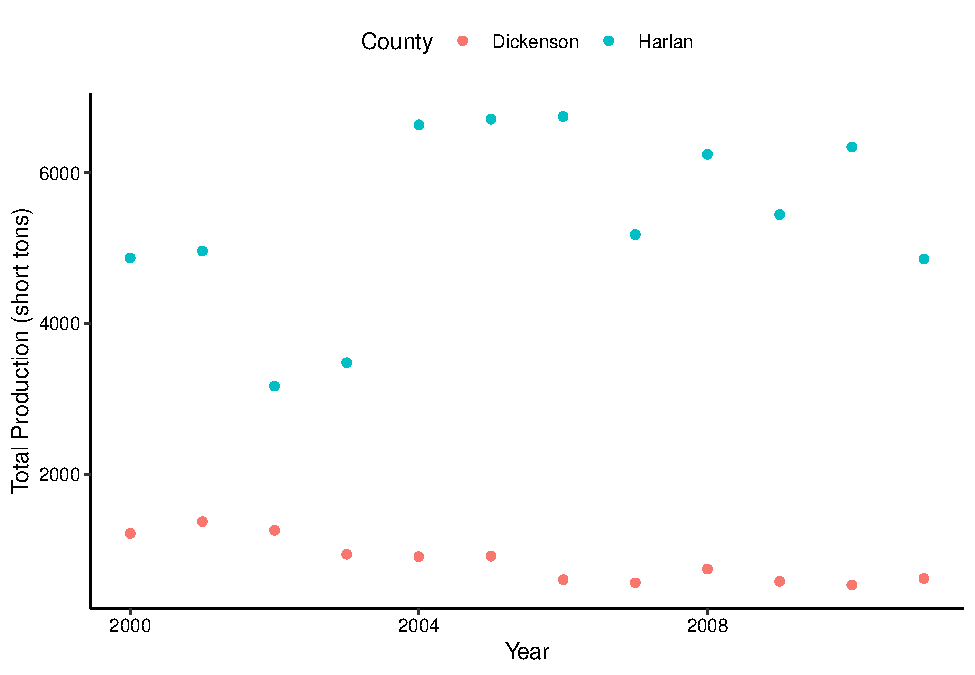
\includegraphics{Smith_ENV872_Project_files/figure-latex/unnamed-chunk-11-1.pdf}
\caption{\label{fig:figs} Total Annual Coal Production in Harlan and
Dickenson Counties by County}
\end{figure}

\begin{figure}
\centering
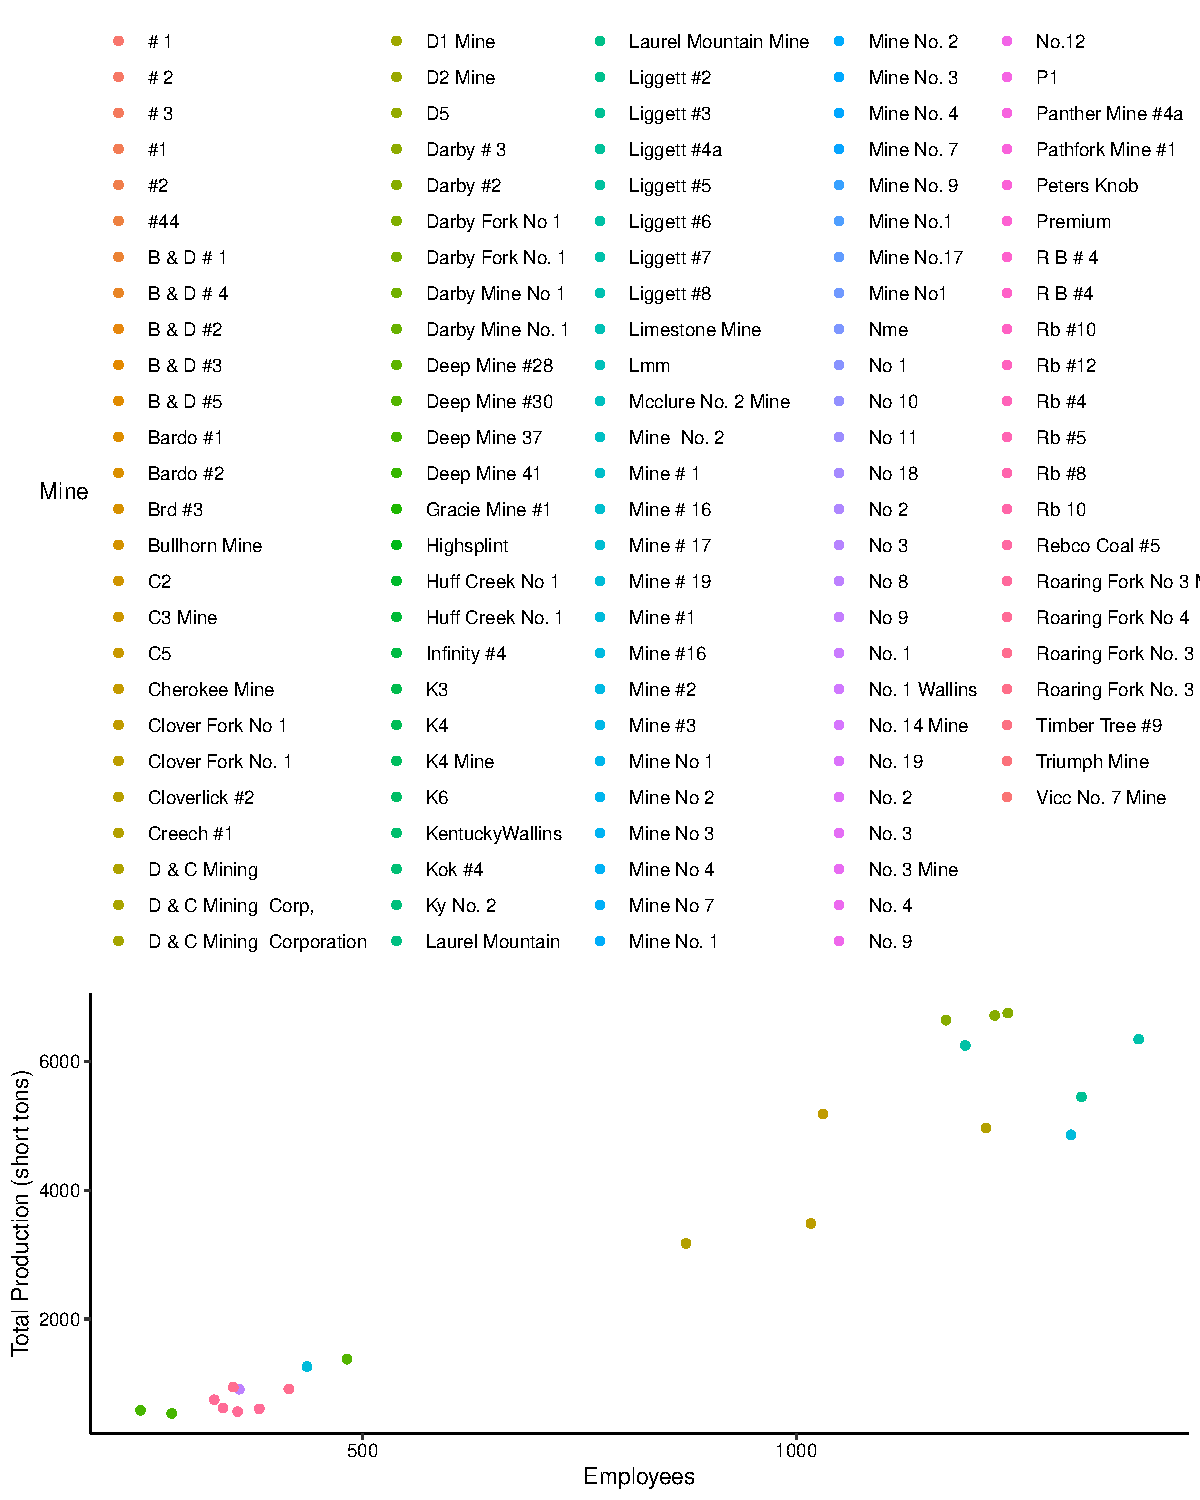
\includegraphics{Smith_ENV872_Project_files/figure-latex/unnamed-chunk-12-1.pdf}
\caption{\label{fig:figs} Total Annual Coal Production versus Total
Employment in Harlan and Dickenson Counties by Mine}
\end{figure}

\begin{figure}
\centering
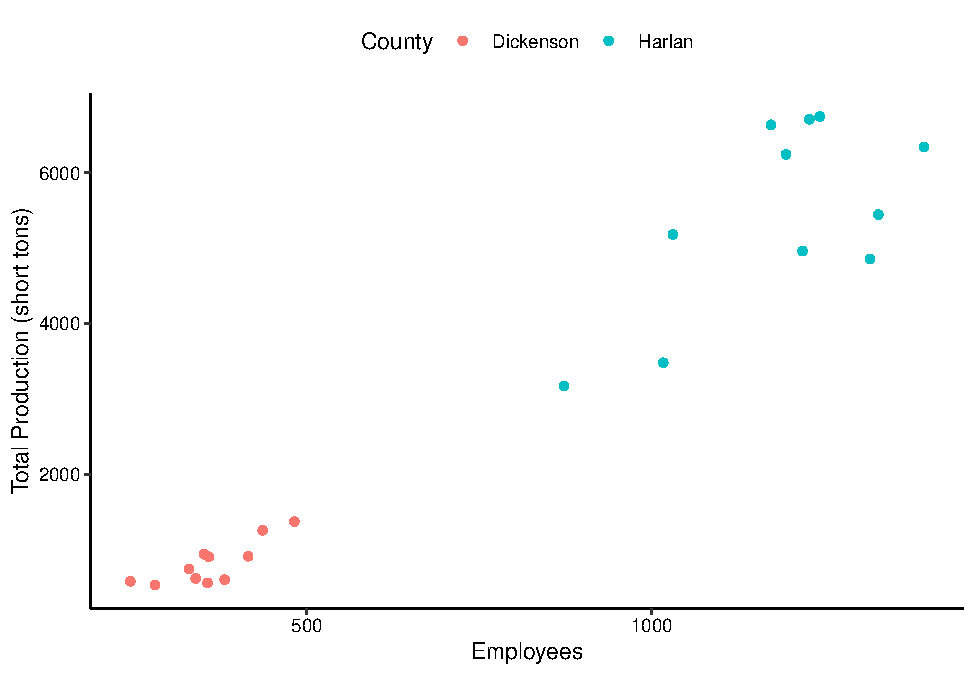
\includegraphics{Smith_ENV872_Project_files/figure-latex/unnamed-chunk-13-1.pdf}
\caption{\label{fig:figs} Total Annual Coal Production versus Total
Employment in Harlan and Dickenson Counties by County}
\end{figure}

The relationship of mines to labor hours, employment, and production
across the coal sector from 2000 to 2011 does not seem to be a
consistent trend, nor is it easy to visualize (Figures 1, 3, and 5).
There are too many mines to determine any sort of relationship;
furthermore, whether a mine is from a boom-bust or bust-bust county is
indeterminable in these visualizations (Figures 1, 3., and 5). However,
mine data for employees related to production shows the most promise for
a significant correlation at the mine level; however, since this project
focuses on coal counties, this correlation is not especially relevant to
the research question (Figure 7).

On the other hand, the exploratory graphs indicate that there are strong
trends in the county-wide data (Figures 2, 4, and 6). Labor hours are
greater than in Harlan than Dickenson on the whole, but do not seem to
display a steady trend through the years (Figure 2). What's interesting
is Harlan appears to have substaintal fluctuations in production through
the years, decreasing quickly in 2002, while Dickenson steadily declined
(Figure 6). Employment seems to follow similar trends for both counties,
but not as drastically (Figure 4). Like the mine level data, both
counties seem to have a strong correlation for employees with total
production (Figure 8).

\newpage

\hypertarget{analysis}{%
\section{Analysis}\label{analysis}}

\hypertarget{what-is-the-relationship-between-coal-production-and-number-of-employees-in-coal-mines-in-harlan-and-dickenson-counties}{%
\subsection{What is the relationship between coal production and number
of employees in coal mines in Harlan and Dickenson
Counties?}\label{what-is-the-relationship-between-coal-production-and-number-of-employees-in-coal-mines-in-harlan-and-dickenson-counties}}

\hypertarget{how-does-coal-production-differ-between-all-mines-in-harlan-county-compared-to-dickenson-county}{%
\subsection{How does coal production differ between all mines in Harlan
County compared to Dickenson
County?}\label{how-does-coal-production-differ-between-all-mines-in-harlan-county-compared-to-dickenson-county}}

\begin{figure}
\centering
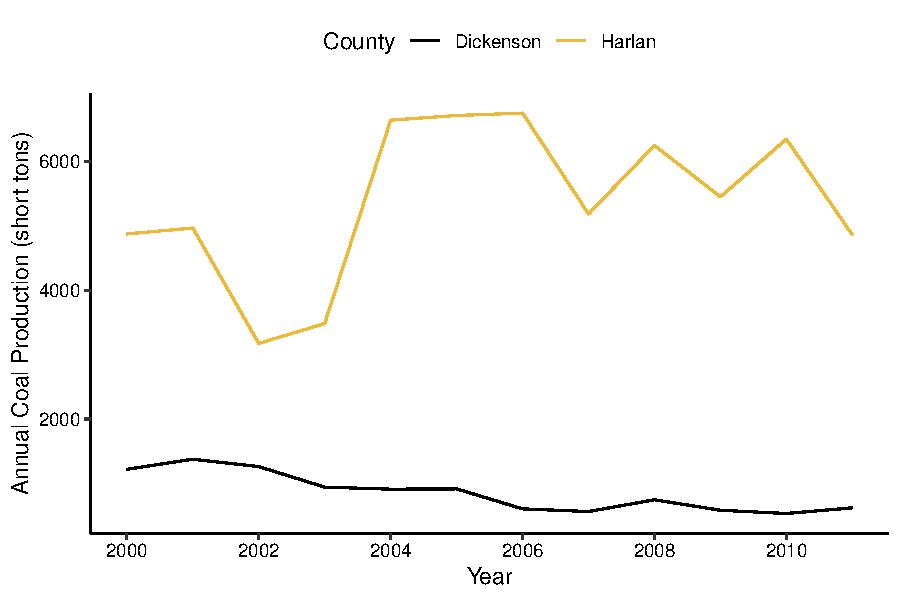
\includegraphics{Smith_ENV872_Project_files/figure-latex/unnamed-chunk-14-1.pdf}
\caption{\label{fig:figs} Total Annual Coal Production in Harlan and
Dickenson Counties}
\end{figure}

\hypertarget{how-does-the-number-of-employees-in-the-mines-of-harlan-county-compare-to-dickenson-county}{%
\subsection{How does the number of employees in the mines of Harlan
County compare to Dickenson
County?}\label{how-does-the-number-of-employees-in-the-mines-of-harlan-county-compare-to-dickenson-county}}

\begin{figure}
\centering
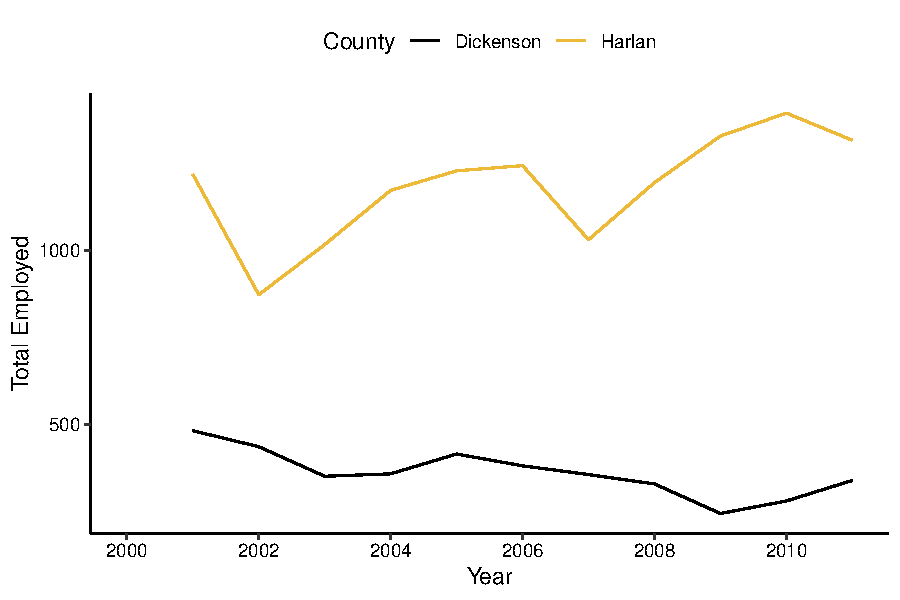
\includegraphics{Smith_ENV872_Project_files/figure-latex/unnamed-chunk-15-1.pdf}
\caption{\label{fig:figs} Total Number of Employees in Harlan and
Dickenson County Mines, 2000 to 2011}
\end{figure}

\hypertarget{is-the-total-number-of-employees-for-all-mines-in-a-boom-bust-and-a-bust-bust-county-in-the-years-2000-to-2011-a-significant-predictor-of-annual-coal-production-for-all-mines}{%
\subsection{Is the total number of employees for all mines in a
boom-bust and a bust-bust county in the years 2000 to 2011 a significant
predictor of annual coal production for all
mines?}\label{is-the-total-number-of-employees-for-all-mines-in-a-boom-bust-and-a-bust-bust-county-in-the-years-2000-to-2011-a-significant-predictor-of-annual-coal-production-for-all-mines}}

\begin{figure}
\centering
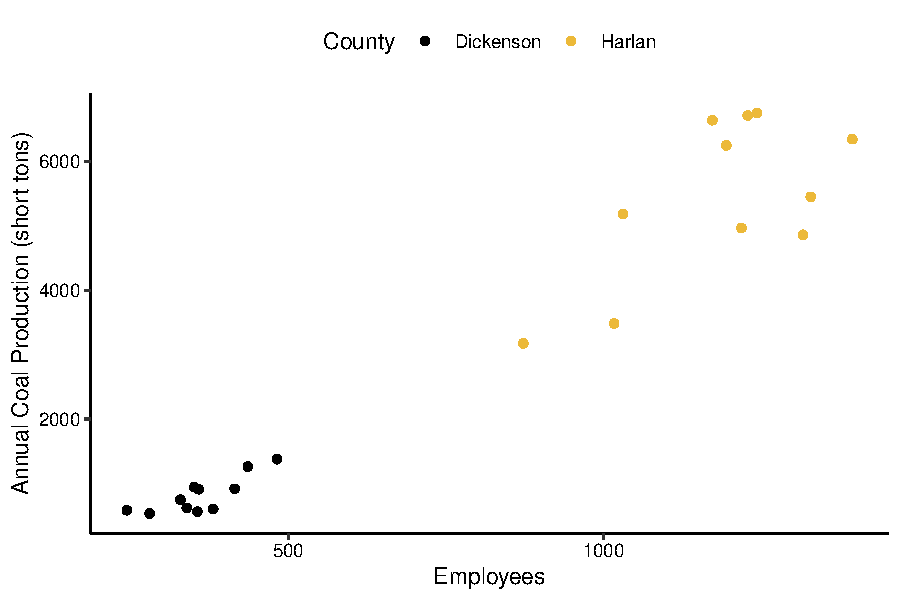
\includegraphics{Smith_ENV872_Project_files/figure-latex/unnamed-chunk-16-1.pdf}
\caption{\label{fig:figs} Annual Coal Production Compared to Total
Employees in Harlan and Dickenson Counties, 2000 to 2011}
\end{figure}

Harlan County, Kentucky produced a much greater amount of coal and
employed more people than Dickenson County, Virginia throughout the
early twenty-first century (Figure 9 and Figure 10). This divergence is
to be expected with Harlan being boom-bust and Dickenson being bust-bust
for coal production 2000 to 2011.

However, Harlan County experienced a variable production amount from
year to year, which is consistent with historical coal production in the
twentieth century (EIA, 2016). Dickenson County, on the other hand,
experienced a steady decline in coal production since 2000 (Figure 9).

Surprisingly, Dickenson also experienced a small increase in coal
employment in 2009 even though there is no coal production increase
during that same time period (Figure 9 and Figure 10). As such, it
becomes essential to question if mine production is an accurate
predictor of mine employment. If so, coal production could be correlated
to migration from an area based on employment.

Although Harlan had more employees and coal production overall than
Dickenson, coal production significantly impacts the number of employees
in mining for both counties (Figure 11; ANOVA; Harlan: df = 288, F =
197.2, p-value \textless{} 0.001; Dickenson: df = 105, F = 276.6,
p-value \textless{} 0.001).

\newpage

\hypertarget{summary-and-conclusions}{%
\section{Summary and Conclusions}\label{summary-and-conclusions}}

Although Harlan and Dickenson counties are both ``coal counties'' within
the scope of this research, Harlan experienced a boom in coal production
in 2000 but a bust in 2010. Dickenson steadidly decreased in that same
time period. However, Harlan had variable coal production and
employment, exhibiting smaller boom-bust cycles within the decade.

Most importantly, both counties' coal production signficantly correlated
with employment in coal mines. Intuitively, this makes sense, as lower
production means less money means less available jobs.

Finally, the correlation between production and employment could be
important for migratory trends in Appalachia. Based on the data in this
research, their are less emplyment opportunities in coal mine with less
coal production. As such, residents of Appalachia may leave the region
in search of jobs as the energy sector slowly transitions from
coal-fired power plants to forms of cleaner energy.

\newpage

\hypertarget{references}{%
\section{References}\label{references}}

EIA. (2020). \textbf{Annual Survey of Coal Production and Preparation;
Form EIA-7A} \url{https://www.eia.gov/survey/form/eia_7a/form.pdf}

EIA. (2016). \textbf{Quarterly coal production since the early 1980s}.
\url{https://www.eia.gov/todayinenergy/detail.php?id=26612}

\end{document}
